\title{Distributed deep learning on biomedical data with Boltzmann machines}
\author{Stefan Lenz}
\date{\today}

\documentclass[12pt]{article}
\usepackage[utf8]{inputenc}
\usepackage{natbib}
\bibliographystyle{abbrvnat}
\usepackage{amsmath}
\usepackage{graphicx}
\usepackage{epstopdf}
\usepackage[table]{xcolor}
\usepackage{tabularx}
\usepackage{makecell}
\usepackage{placeins}
\usepackage{setspace}
\usepackage[a4paper,bindingoffset=0.2in,%
            left=2.8cm,right=2.8cm,top=2.1cm,bottom=2.8cm,%
            footskip=.25in]{geometry}
\usepackage{helvet}
\renewcommand{\familydefault}{\sfdefault}

\newcommand{\inlinecode}[1]{\texttt{#1}}
\newcommand{\sigm}{\mathrm{sigm}}


\begin{document}

%\maketitle

\tableofcontents
\newpage
\onehalfspacing

\begin{abstract}
We present the Julia package ``BoltzmannMachines.jl" that provides a friendly interface to algorithms for training and evaluating Boltzmann machines.
The ability of Boltzmann machines to deal with rather small sample sizes makes them especially interesting for analyzing medical data sets. But since these data sets can be very heterogeneous compared to the widely used image data, the choice of hyperparameters for training is especially challenging.
Therefore the package puts a strong focus on monitoring and evaluating the learning process.
Primary evaluation criterion is the likelihood of the model, which can be estimated using annealed importance sampling (AIS). We present our approach for adapting the AIS algorithm on multimodal deep Boltzmann machines in detail in the article.
Additionally to likelihood estimation, this package offers convenience methods to monitor a number of other statistics and it allows to easily extend the monitoring of the training.
\end{abstract}

\section{Introduction}
Multimodal DBMs have been used by Srivastava et al. for image captions \citep{srivastava2012multimodal}.
Here we want to broaden the scope a little bit and present an extensible approach for creating deep Boltzmann architectures with different types of visible units and flexible partitioned hidden layers. Training of such architectures ....
Those architectures are not only useful for putting data of different types in one model but also in cases where a natural partitioning of the data can be derived from domain knowledge. With partitioning one can greatly reduce the number of parameters in the model. This allows training models on data sets where the sample size would otherwise be too small to fit a full model.
Hess et al. showed that partitioned training on genetic data is successful \citep{hess2017partitioned}.

A special challenge for unsupervised learning on non-image data is the lack of performance indicators.
In supervised training, the classification accuracy is the natural evaluation criterion, which is also easy to implement.
In unsupervised training with a well investigated class of data such as images, there is already much experience available for choosing the model architecture and the hyperparameters. If models are to be trained on very diverse data, the problem of finding good hyperparameters is exacerbated as for each data set the challenge of tuning can pose a different challenge.

Thus the need for having an objective evaluation criterion as a basis for choosing the hyperparameters and monitoring the training becomes very important.
In case of images or natural language, the generative abilities of a model can be tested by simply looking at the generated images or sentences to see whether these are proper samples. In the case of data from a patient record or genetic data, this approach is not feasible. As the best indicator for successful learning,which is applicable in all cases of data, remains the model likelihood. In most cases, the likelihood cannot be calculated exactly but it can only be estimated by stochastic algorithms like annealed importance sampling (AIS). So we also want to detail the extension of AIS on multimodal deep Boltzmann machines in this article.

For the implementation we chose the Julia language \citep{bezanson2017julia}. % TODO elaborate or remove

\section{Methods}

\subsection{Basic properties of Boltzmann machines}

A Boltzmann machine model with parameters $\Theta$ defines a probability distribution $p(x)$ for a random variable $x = (v, h)$ in a probability space $\Omega$ via an energy function $E(v, h; \Theta)$:
\[
   p(x) = p(v, h) = \frac{e^{-E(v,h)}}{Z}.
\]
The normalizing factor $Z$, the so called \emph{partition function}, is defined as $Z = \int_{\Omega} e^{-E(x)} dx$. In case of a discrete probability distribution, this can be written as $Z = \sum_{v,h}e^{-E(v,h)}$ where the sum goes over all possible combinations of $v$ and $h$.
The term in the denominator $p^*(v,h) = e^{-E(v,h)}$ is called \emph{unnormalized probability}.
The probability space is divided into dimensions of observed variables (subsumed in vector $v$) and hidden/latent variables (in $h$), corresponding to visible and hidden nodes in the graphical representation, see figure TODO Bild.

The so called \emph{free energy}, a notation inspired by physics, is defined as
\[
   F(v) = - \log \sum_h e^{-E(v, h)}
\]
This allows rewriting the formula of the logarithmized partition function as $Z = \sum_v e^{-F(v)}$.
That is useful because the formula for the free energy of restricted Boltzmann machines can be simplified by using the layerwise structure.
Thus the complexity of calculating the free energy becomes linear in the number of hidden nodes. (This can be seen in the formulas for the free energy in the different types of models that are described below.)
This way the log-likelihood
\begin{equation}
   \log p(v) = - F(v) - \log Z
\label{eqpRBMfreeenergy}
\end{equation}

can be calculated efficiently if the partition function $Z$ is given. The free energy is also used for calculating the ratio of the unnormalized probabilities $p^*(v) = e^{-F(v)}$ in the annealed importance sampling algorithm (see \ref{methodAIS}).

\subsection{Subtypes of Boltzmann machines}

Here we only consider the special cases of restricted Boltzmann machines and (multimodal) deep Boltzmann machines.
These models have restrictions on their parameterization, corresponding to a layered design of their graphs.

\begin{figure}[h]
   \centering
   
\includegraphics[scale=3.]{images/BMsOverview.eps}
   \caption{Different types of Boltzmann machines}
 \end{figure}


\subsubsection{Bernoulli distributed visible nodes}
The most basic model in this class of models are restricted Boltzmann machines with Bernoulli distributed nodes, most of the time simply called \emph{restricted Boltzmann machines} (RBMs). The energy function is of the form
\[
   E(v,h) = a^T v + b^T h + v^T W h.
\]
The parameters of this model are $\Theta = (W, a, b)$ with \emph{weight matrix} $W$, vector $a$ as the \emph{visible bias} and $b$ as the \emph{hidden bias}.
Employing the sigmoid function $\sigm(x) = \frac{1}{1+ e^{-x}}$, the resulting conditional distributions can be written as $p(v_i | h) = \sigm ((a + W h)_i)$ and $p(h_i | v) = \sigm ((b + W^T v)_i)$. The free energy is
\[
F(v) = - a^T v - \sum_{j=1}^{n_H} \log \left (1 + e^{(W^T v + b)_j}\right).
\]

\subsubsection{Continuously valued visible distributions}
One way of modeling continuous values for $v$ are restricted Boltzmann machines with Gaussian distribution of the visible variables and Bernoulli distributed hidden variables. The energy of the model is defined as
\[
   E(v,h) = \sum_{i=1}^{n_V}\frac{(v_i - a_i)^2}{2\sigma_i^2} - b^T h - \sum_{i=1}^{n_V} \frac{(Wh)_i}{\sigma_i}
\]
The number of visible and hidden nodes is denoted as $n_V$ and $n_H$, respectively. The parameters of this model are $\Theta = (W, a, b, \sigma)$ with weight matrix $W$, visible bias $a$ hidden bias $b$ and standard deviation $\sigma$. The role of $\sigma$ as standard deviation becomes clearer by looking at the conditional distributions of the $v_i$ given $h$, which are distributed according to the normal distribution $\mathcal{N}(a_i + \sigma_i(Wh)_i, \sigma_i^2)$. For the hidden nodes, $p(h_j | v) = \sigm \left (b_j + \sum_{i=1}^{n_V} w_{ij} \frac{v_i}{\sigma_i} \right )$.
The free energy is
\[
   F(v) = \sum_{i=1}^{n_V}\frac{(v_i - a_i)^2}{2\sigma_i^2} + \sum_{j=1}^{n_H} \log \left (1 + e^{b_j + \sum_{i=1}^{n_V} \frac{v_i}{\sigma_i} w_{ij}} \right).
\]
\citep{krizhevsky2009tinyimages}.

Cho et al. \citep{cho2011improved} proposed a different parameterization for the energy function:
\[
   E(v,h) = \sum_{i=1}^{n_V}\frac{(v_i - a_i)^2}{2\sigma_i^2} - b^T h - \sum_{i=1}^{n_V} \frac{(Wh)_i}{\sigma_i^2}
\]
In this model the distribution of the visible nodes is the multimodal normal distribution $\mathcal{N}(a + Wh, \sigma^2)$.
The conditional distribution of the hidden nodes is $p(h_j | v) = \sigm \left (b_j + \sum_{i=1}^{n_V} w_{ij} \frac{v_i}{\sigma_i^2} \right )$.

\subsubsection{Multimodal deep Boltzmann machines}

The energy function of a multimodal deep Boltzmann machine (MDBM) is


\subsection{Training}

TODO stochastic gradient descent, batch gradient descent, minibatches \citep{bengio2012practical}
contrastive divergence, persistent contrastive divergence

For pre-training the multimodal deep Boltzmann machines, we use greedy layerwise pre-training of layers of restricted Boltzmann machines.
Fine-tuning of weights can then be performed by the algorithm for training a general Boltzmann machine.
\citep{salakhutdinov2009DBMs}, \citep{salakhutdinov2015generativemodels}

When training with the mean-field approximation $\mu$ used as activation of the hidden nodes in the positive phase,
the likelihood is not optimized directly but a lower bound
\[
   \log p(v) \geq - E(v, \mu) - \log Z + \mathcal{H}(\mu)
\]
is optimized. $\mathcal{H}$ denotes the entropy of the hidden nodes. \citep{sala2012anefficient}

TODO stacking
TODO Bild von multimodal
TODO Referenz zu Srivastava

\subsection{Evaluating}

\subsubsection{Exact calculation of the partition function}
\label{methodExactloglik}
The exact calculation of partition functions is only computationally feasible for very small models as its complexity grows exponentially. Exploiting the layerwise structure allows a faster exact calculation of $Z$ such that the computation time does not grow exponentially with the number of all nodes but only grows exponentially with the number of elements in a subset of the nodes. That means, the complexity is still $\mathcal{O}(2^n)$, but with an $n$ smaller than the number of nodes.
By using the formulas for the free energy and the symmetry of restricted Boltzmann with binary nodes, $n = \min(n_V, n_H)$.
In RBMs with one of layer Gaussian nodes and one layer of binary nodes, $n$ is the number of binary nodes, since the contribution of the Gaussian nodes can be integrated analytically.
In case of a deep Boltzmann machine, it is possible to sum out each second layer, similar to the calculation of the free energy in restricted Boltzmann machines. So for DBMs, $n$ can be reduced to the number of nodes in each second layer.

\subsubsection{Estimating partition functions with annealed importance sampling (AIS)}\label{methodAIS}

For annealed importance sampling we need a sequence of intermediate distributions
$p_0, \dots p_K$ with
$p_0 = p_A$ and $p_K = p_B$. The ratio $\frac{Z_B}{Z_A}$ is then estimated by the mean of a number of so called importance weights that are determined as
\[
   \prod_{k=1}^K \frac{p^*_k(x_k)}{p^*_{k-1}(x_{k-1})}.
\]
The $x_k$ are produced by iteratively performing Gibbs sampling. Starting with $x_0$ sampled from $p_0$, one obtains $x_k$ by sampling a Gibbs chain that is initialized with $x_{k-1}$ in an intermediate model with distribution $p_k$. An appropriate choice for the intermediate models are Boltzmann machines with the energy functions $E_k$ chosen such that
\[
   E_k(x) = (1 - \beta_k) E_A(x) + \beta_k E_B(x)
\]
and therefore
\[
   p_k^*(x) = p_A^*(x)^{1-\beta_k} p_B^*(x)^{\beta_k}.
\]
The factors $\beta_k$ with $0 = \beta_0 < \beta_1 < ... < \beta_K = 1$ are called temperatures. \citep{salakhutdinov2008learning}
The choice of the temperatures, the number of importance weights and also the number of Gibbs sampling steps for the transition are hyperparameters for the AIS algorithm.

There are two practical approaches for constructing intermediate models with such a distributions (see also figure \ref{figTwotypesais}):
\begin{enumerate}
\item Combine corresponding weights of two models of the same size to get an intermediate model of the same size.
\item Constructing a larger model by putting the two models next to each other and connecting their nodes, increasing the energy in one part of the combined model while reducing it in the other part. \citep{theis2011deepbelief}
\end{enumerate}
\begin{figure}[h]
\centering

\includegraphics[scale=3.]{images/twotypesais.eps}
\caption{The two approaches for AIS, sketched for restricted Boltzmann machines.
The weights of the first model are shown depicted as continuous lines, the weights of the second as dashed lines. The tempered weights of the intermediate distributions are shown in grey.}
\label{figTwotypesais}
\end{figure}
The second approach is more flexible and allows to estimate the ratios of two arbitrary Boltzmann machines of the same type and with the same number of hidden nodes. But it requires sampling in a Boltzmann machine that has as many hidden nodes as the two models together.
Both approaches can be used to estimate the partition function of a single Boltzmann machine by estimating the ratio of the model's partition function to the partition function of a base rate model with known partition function.


\subsubsection{Calculating or estimating likelihoods} %TODO verbessern
For a restricted Boltzmann machine, the likelihood can be calculated using formula (\ref{eqpRBMfreeenergy}) if the partition function is known. This is not so easily possible in a DBM, for which calculating the distribution of the hidden nodes is of exponential complexity.
Estimating the likelihood of DBMs is possible using AIS by constructing a smaller DBM for each sample and estimating its partition function.
The smaller DBM is constructed by removing the visible layer, and incorporating contribution of the sample to the energy of the first RBM - consisting only of visible and first hidden layer - into the bias of the new visible layer which was the first hidden layer of the original model.
The partition function of this smaller model is then the unnormalized probability of the sample in the original model.
In a setting with very large sample size, the cost of estimating the actual likelihood with this procedure is too expensive. But if the sample size is smaller, it is affordable to estimate the likelihood and not fall back on the lower bound.

\section{Results}

\subsection{Example}

TODO describe example data set.

The following lines of code shows how a multimodal deep boltzmann machine is trained.

\subsection{Modelling}

In our implementation multimodal deep Boltzmann machines, corresponding to the type \inlinecode{MultimodalDBM}, are constructed using restricted Boltzmann machines as building blocks (see figure \ref{mdbmimplasstack}). For each of the models of Boltzmann machines, it is possible to generate samples by using Gibbs sampling. For efficiently evaluating very small models, the likelihood and the partition function can be calculated exactly. This is also useful to test AIS by comparing the values estimated in small models to the exact ones.

\begin{figure}[h]
   \centering
   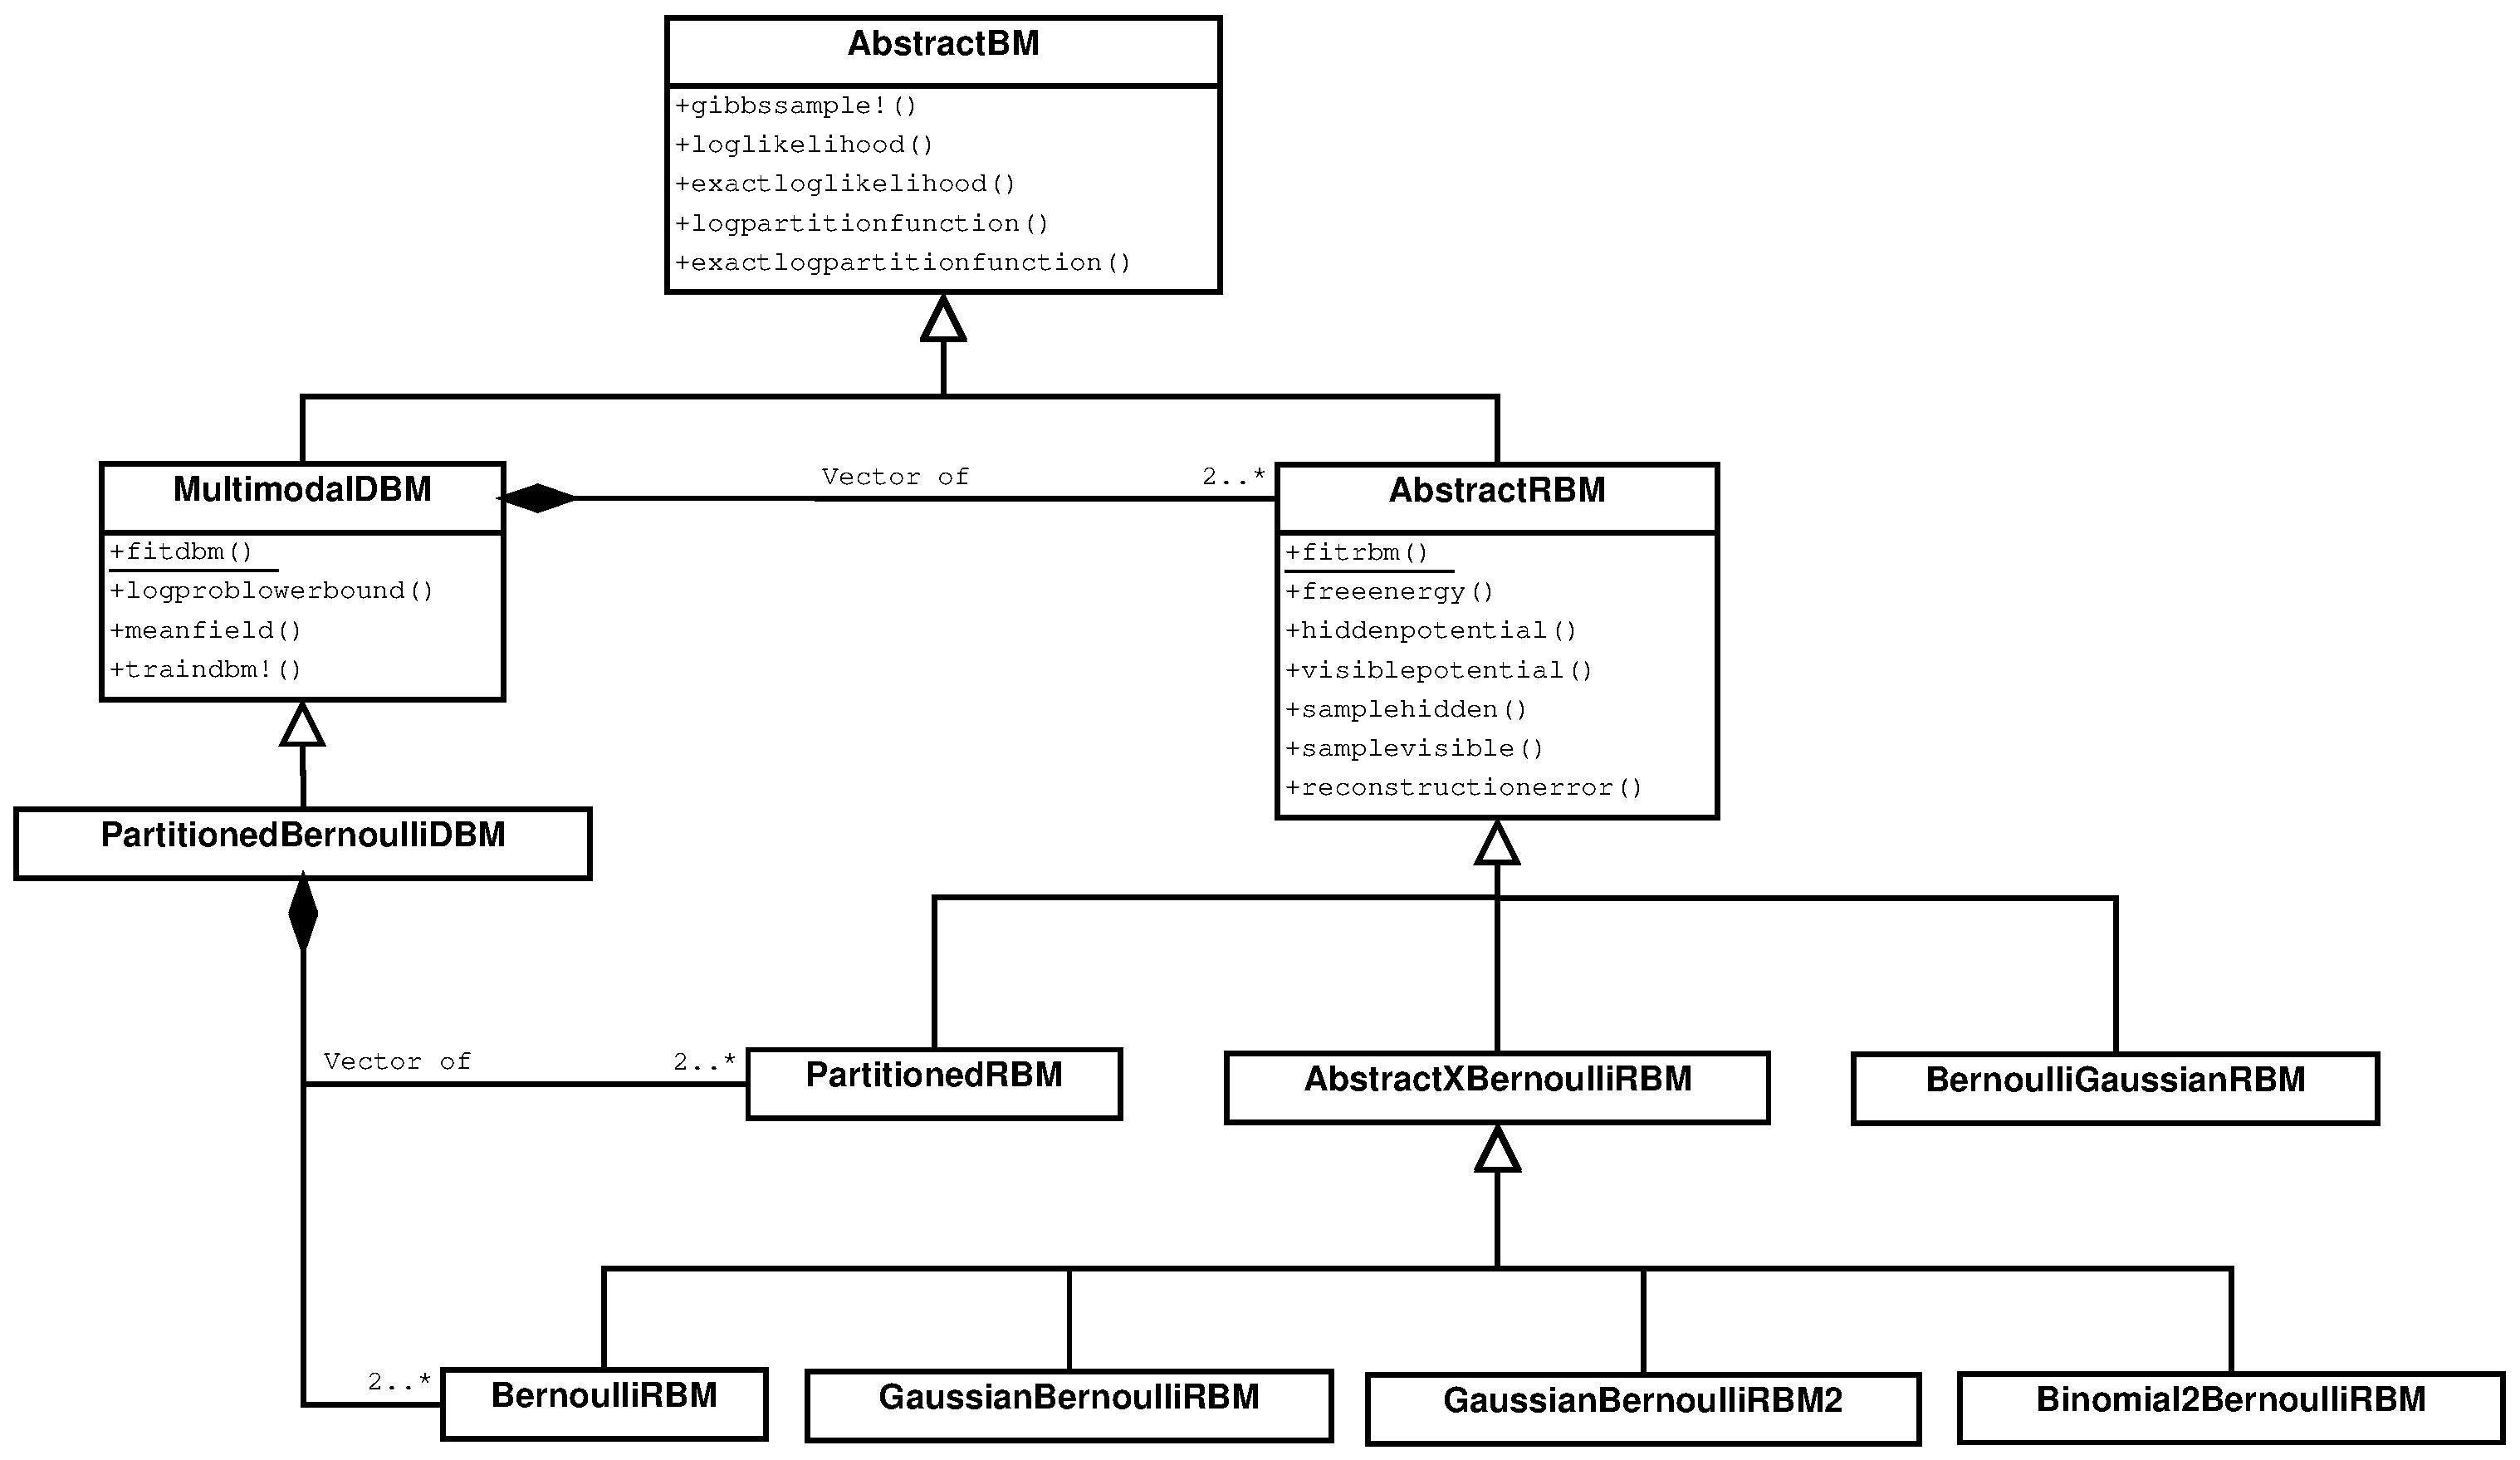
\includegraphics[scale=0.25]{images/BoltzmannMachinesDiagram.eps}
   \caption{UML class diagram \citep{uml} of the type hierarchy for the Boltzmann machines in our Julia implementation. Although the Julia language does not have the concept of classes and visibility, the diagram is suited well to show the connections of the types with the most important associated functions.
   For more details on these functions, see tables \ref{juliaFunTableTrain} and \ref{juliaFunTableEval}.}
   \label{umlclassdiagram}
\end{figure}

\begin{figure}[h]
   \centering
   
\includegraphics[scale=3.]{images/MDBMImpl.eps}
   \caption{Multimodal deep Boltzmann machines are modeled as a stack of restricted Boltzmann machines. On the left hand side an example model is depicted as a graph and on the right hand side the corresponding modelling in the Julia package is shown.
   The first/lowest and the second layer are modelled as a \inlinecode{PartitionedRBM}s (white boxes with grey borders), each containing a vector holding two \inlinecode{BernoulliRBM}s (grey filled boxes).
   The third/highest layer is simply a \inlinecode{BernoulliRBM}.
   All three \inlinecode{AbstractRBMs} in a vector form the \inlinecode{MultimodalDBM}.
   The arrows indicate the ordering of the vectors.}
\label{mdbmimplasstack}
\end{figure}


\rowcolors{1}{gray!25}{white} % alternating row colors in tables
\begin{table}
\begin{tabularx}{\textwidth}{X}
   \hline
   \inlinecode{fitrbm(x;...)} \\
   Fits a restricted Boltzmann machine model for a given data set \inlinecode{x} and additional model hyperparameters \\
   \inlinecode{fitdbm(x; ...)} \\
   Fits a (multimodal) deep Boltzmann machine model for a given data set \inlinecode{x} and model hyperparameters \\
   \inlinecode{meanfield(dbm, x)} \\
   Calculates the mean-field activations of the \inlinecode{dbm}'s hidden nodes given the activations of the visible nodes \inlinecode{x}. \\
   \inlinecode{stackrbms(x;...)} \\
   Pre-trains a stack of RBMs on a given data set \inlinecode{x}. It can either be used for pre-training of a DBM or to train a deep belief network. \\
   \hline
\end{tabularx}
\caption{Functions in the Julia package for training}\label{juliaFunTableTrain}
\end{table}

\rowcolors{1}{gray!25}{white}
\begin{table}
   \begin{tabularx}{\textwidth}{X}
   \hline
   \inlinecode{logpartitionfunction(bm; ... )} \\
   Estimates log of the partition function of the Boltzmann machine \inlinecode{bm} using AIS. Additional hyperparameters for AIS may be provided. \\
   \makecell[tl]{
      \inlinecode{loglikelihood(rbm, x)} \\
      \inlinecode{loglikelihood(rbm, x, logz)}
   } \\
   Calculates the log-likelihood of data \inlinecode{x} in the restricted Boltzmann machine model \inlinecode{rbm}. The log of the partition function can be provided as parameter \inlinecode{logz} or is estimated using AIS. \\
   \makecell[tl]{
      \inlinecode{loglikelihood(dbm, x; ...)} \\
      \inlinecode{loglikelihood(dbm, x, logz; ...)}
   } \\
   Estimates the log-likelihood of a (multimodal) deep Boltzmann machine using AIS for each sample. Additional hyperparameters for AIS may be provided. \\
   \inlinecode{logproblowerbound(dbm, x; ...)} \\
   Estimates the stochastic lower bound of the log-likelihood that is optimized by the training algorithm with mean-field optimization. \\
   \inlinecode{exactloglikelihood(bm, x)} \\
   Calculates the log-likelihood of a deep Boltzmann machine. \\
   \inlinecode{exactlogpartitionfunction(bm, x)} \\
   Calculates the log of the partition function for a restricted Boltzmann machine. \\
   \hline
\end{tabularx}
\caption{Functions in the Julia package for evaluating the likelihood of trained models. The exact calculations of the partition function and the likelihood are only feasible for very small models. For the complexity of the corresponding algorithms, see \ref{methodExactloglik}.}
\label{juliaFunTableEval}
\end{table}

\FloatBarrier
\subsection{Training algorithm and choices of hyperparameters}

TODO minibatch - nicht nur für performance

TODO GaussianRBMs

\subsection{Implementation of annealed importance sampling}

Like described by Salakhutdinov et al. \citep{salakhutdinov2008learning}, we use only the states of each second layer from samples generated by running a Gibbs chain. The unnormalized probabilities of these states can be calculated by analytically summing out the other layers.
In a \inlinecode{MultimodalDBM}, we use the fact that the states in one layer are independent from the states of each non-adjacent layer to get $p^*(\tilde{x}) = p^*(h^{(1)}) \cdot p^*(h^{(3)}) \cdot \dots $ as unnormalized probability for the subset $\tilde{x} = (h^{(1)}, h^{(3)}, \dots)$ of a generated sample $x = (v, h^{(1)}, h^{(2)}, \dots)$.
For generalizing the implementation of AIS on multimodal deep Boltzmann machines, additional to summing out intermediate Bernoulli distributed layers or the top layer, it then is sufficient to provide the function for calculating $p^*(h)$ for each type of RBM that is usable as bottom RBM in a \inlinecode{MultimodalDBM}.

Due to the symmetry of hidden and visible nodes in a RBM with only Bernoulli distributed nodes, $p^*(h)$ can be derived analogously to the free energy $F(v) = - \log p^*(v)$ in this case.
The unnormalized probability of the hidden nodes in a \inlinecode{GaussianBernoulliRBM} (original parameterization) can be derived as

\begin{align*}
   p^*(h) &= \int e^{-E \left(v,h \right)} dv \\
   &= \int \exp \left( -\sum_{i=1}^{n_V}\frac{(v_i - a_i)^2}{2\sigma_i^2} + b^T h + \sum_{i=1}^{n_V} \sum_{j=1}^{n_H} \frac{v_i}{\sigma_i}h_j w_{ij} \right) dv\\
   &= e^{b^T h} \int \exp \left( \frac{v_i^2 -2 a_i v_i + a_i^2 - 2 v_i (Wh)_i \sigma_i}{2 \sigma_i^2} \right) dv \\
   &= e^{b^T h} \int \exp \left(
      - \sum_{i=1}^{n_V} \frac{{\left( v_i - \left( (Wh)_i \sigma_i + a_i \right) \right)}^2}{2\sigma_i^2} + \frac{1}{2}(Wh)_i^2 + (Wh)_i \frac{a_i}{\sigma_i} \right ) dv \\
   \begin{split}
      &= \exp \left(b^T h + \sum_{i=1}^{n_V} \frac{1}{2}(Wh)_i^2 + (Wh)_i \frac{a_i}{\sigma_i} \right ) \cdot \\
      & \quad \quad \int \exp \left ( - \sum_{i=1}^{n_V} \frac{{\left( v_i - ((Wh)_i \sigma_i + a_i) \right)}^2}{2\sigma_i^2} \right) dv
   \end{split} \\
   & = \exp \left( b^T h + \sum_{i=1}^{n_V} \frac{1}{2}(Wh)_i^2 + (Wh)_i \frac{a_i}{\sigma_i} \right ) \prod_{i=1}^{n_V}\left(\sqrt{2\pi} \sigma_i\right). \\
\end{align*}

For the \inlinecode{GaussianBernoulliRBM2} (with Cho's alternative parameterization), the unnormalized probability calculates analogously as
\[
   p^*(h) = \exp \left( b^T h + \sum_{i=1}^{n_V} \frac{\frac{1}{2}(Wh)_i^2 + (Wh)_i a_i}{\sigma_i^2} \right ) \prod_{i=1}^{n_V}\left(\sqrt{2\pi} \sigma_i\right).
\]

Note that the model for Gibbs sampling, used as the Markov transition operator, can differ from the model that is used to evaluate the unnormalized probability $p_k^*(h)$ as long as the probability distribution $p_k(h)$ of the hidden nodes is the same.
This trick can be used to fit AIS for GBRBMs in the same schema as RBMs with Bernoulli distributed nodes.


\subsection{Monitoring: Evaluation during the training process}



The hyperparameters for layerwise pre-training can be defined for the whole network or for each layer separately. %TODO Trainlayer, AbstractTrainLayer.

TODO cross validation

\section{Discussion}

For large datasets such as image collections from the internet, optimizing the execution speed is essential.
Popular libraries like TensorFlow \citep{abadi2016tensorflow}, MXNet \citep{mxnet} and PyTorch \citep{pytorch} work with abstraction of the computations on tensors (multidimensional matrices) with so called computational graphs.
This way the computations can be performed on the CPU as well as on the GPU.
The high parallelization in GPUs can bring far greater performance while at the same time it requires a high sophistication of the code to fully exploit the advantages of GPUs and port the algorithms to their SIMD (single instruction multiple data) architecture.
In order to work with the abstraction, users must learn this new programming style. Extending and modifying the algorithm and is comparatively hard, especially while trying to maintain the speed benefits of the frameworks.
In contrast to that, we used plain Julia code because we wanted to have an easy access to the code to be able to tailor the algorithms to our needs and experiment with modifications.
Optimizing code by using parallel execution is also possible with the Julia language although, of course, not on the same level.
Since the multiplication of large matrices is already threaded by the linear algebra library called by Julia,
the easiest reduction of execution time can be achieved by reusing allocated space as much as possible.
With the function \inlinecode{mul!} instead of the normal matrix multiplication operator (\inlinecode{*}), it is possible to perform matrix multiplication in-place, without allocating space for the result. Avoiding the costs of memory allocations and garbage collection this way greatly increased the speed in many parts of the code.
In the current version of Julia, explicit control over multi-threading is still an experimental feature and the main way to parallelize is by starting processes.
Sharing memory between processes is more difficult than sharing memory between threads. Also starting processes is more expensive than starting threads.
But with matured multi-threading in Julia, these problems could be solved in the future and e. g. computations on different layers of a deep Boltzmann machine could be done in parallel threads without making the code much more complex.

% TODO for our purposes, the speed was sufficient, especially for smaller models not relevant.


\bibliography{references}


\end{document}